%=========================================================
\chapter{Diseño de acuerdo a la metodología elegida}
\label{cap:reqUsr}

	En este capítulo se modela el alcance del sistema. Se presentan inicialmente los Actores involucrados y sus requerimientos, especificando cuales se alcanzaron en la primera iteración y cuales serán trabajados en la segunda iteración. Después se presentan los requerimientos funcionales de esta iteración y al final se presenta el modelo Físico y Lógico del sistema.


%---------------------------------------------------------
\section{Metodología de desarrollo} 
La metodología a utilizada fue el modelo incremental, debido a que nos permite tener prototipos del proyecto los cuales suelen mostrarse en incrementos, los cuales conllevan análisis, diseño, codificación y pruebas, Con esto se mantiene en constante contacto con los resultados obtenidos en cada uno de ellos. 
 
No solo presenta esas ventajas si no conlleva otras como las siguientes: 

\begin{itemize}
\item Los incrementos son pequeños. 

\item Permite una fácil administración de las tareas en cada iteración. 

\item La inversión se materializa a corto plazo. 

\item Es un modelo propicio a cambios o modificaciones. 

\item Se adapta a las necesidades que surjan. 
\end{itemize}

Para que esto sea posible, se debe tener en cuenta que las iteraciones no pueden ser demasiado rígidas y que no existan tareas simultáneas. El modelo incremental exige un encadenamiento progresivo de cada tarea. Scrum y Kanban son las herramientas más conocidas que emplean este modelo de gestión. \cite{GrandesErrores}


%---------------------------------------------------------
\section{Metodología de desarrollo} 
La solución es crear una aplicación web la cual se encargará de la gestión de proyectos. Para dicha herramienta se leyó sobre las diferentes metodologías desde las ágiles hasta las pesadas, con ello se analizó y diseño la aplicación que pudiera adaptarse alguna de las leídas, y el flujo de trabajo será independiente de la metodología a utilizar. 

 La aplicación busca que, durante la planeación del proyecto, esta pueda ofrecer las recomendaciones de los usuarios registrados en la misma aplicación. Para cuando un líder busque colaboradores, la aplicación le muestra a través de un algoritmo, las sugerencias de colaboradores con ciertos roles que él necesite para poder invitar al proyecto del líder, esto con el fin de que el líder de proyecto pueda escoger a los colaboradores que tengan un buen desempeño, esto teniendo base a proyectos en los que dichos colaboradores hayan participado. 

 Con lo anterior mencionado se espera ahorrar tiempo de planeación de quienes serán los que participaran en dicho proyecto, así el líder de proyecto podrá tener algo de fiabilidad de con quien estará trabajando durante el proyecto que esté en curso. 

%---------------------------------------------------------
\section{Objetivos Generales }

Nuestra herramienta web multiplataforma tiene como objetivo brindar elementos al líder de un proyecto de software en la planeación, gestión y desarrollo del proyecto para una mejor toma de decisiones, concentrando en ella información actualizada del estado del proyecto. 


%---------------------------------------------------------
\section{Objetivos Específicos}

Lograr que la aplicación pueda sugerir al personal a utilizar en los proyectos de la empresa, mediante un algoritmo que evalúe el desempeño de los colaboradores, y con ello puedan ser sugeridos como nuevos colaboradores en algún proyecto a realizar. 

\section{Requisitos Funcionales}
\begin{itemize}
\item La aplicación debe iniciar sesión. 

\item La aplicación debe permitir crear una cuenta. 

\item La aplicación debe permitir recuperar la contraseña. 

\item La aplicación debe permitir gestionar proyectos. 

\item La aplicación debe permitir crear un nuevo proyecto. 

\item La aplicación debe permitir editar un proyecto. 

\item La aplicación debe permitir eliminar un proyecto. 

\item La aplicación debe permitir colocar un proyecto en pausa. 

\item La aplicación debe permitir cerrar un proyecto. 

\item La aplicación debe permitir colocar una descripción de por qué se cierre un proyecto. 

\item La aplicación debe permitir visualizar los datos de un proyecto. 

\item La aplicación debe permitir visualizar las tareas de un proyecto. 

\item La aplicación debe permitir crear una tarea nueva a un proyecto. 

\item La aplicación debe permitir editar una tarea del proyecto. 

\item La aplicación debe permitir asignar una tarea a un colaborador. 

\item La aplicación debe permitir invitar un colaborador dando su correo electrónico. 

\item La aplicación debe permitir invitar a un colaborador previamente registrado en el sistema. 
\end{itemize}

\section{Requisitos No Funcionales }
\begin{itemize}
\item Usabilidad: con ello se busca que la aplicación sea amigable para los usuarios que a utilicen y no sea tedioso el proceso de gestión de su proyecto. 

\item Mantenibilidad: con esto se busca que la aplicación pueda ser susceptible a actualizaciones que ayuden al rendimiento de la aplicación. 

\item Seguridad: con ello se busca que la aplicación mantenga los datos de los proyectos del usuario de forma confidencial, que no pueda ser modificada por un tercero. 
\end{itemize}


%---------------------------------------------------------
\begin{Usuario}{\subsection{Usuario}}{
	Es aquel actor que no se encuentra registrado en el sistema. 
}
    \item[Responsabilidades:] \cdtEmpty
    \begin{itemize}
		\item Registrarse en la plataforma 
    \end{itemize}

	\item[Perfil:] \cdtEmpty
    \begin{itemize}
		\item Persona que aún no se encuentra registrada en la plataforma  
    \end{itemize}
\end{Usuario}

%---------------------------------------------------------
\begin{Usuario}{\subsection{Líder de proyecto }}{
	Es el actor con la capacidad para crear un proyecto, asignar tareas, invitar colaboradores, designar responsables y hacer el seguimiento del proyecto.
}
    \item[Responsabilidades:] \cdtEmpty
    \begin{itemize}
		\item Crear un proyecto 

		\item Asignar tareas a un proyecto 

		\item Asignar responsables a una tarea 
    \end{itemize}

	\item[Perfil:] \cdtEmpty
    \begin{itemize}
		\item Persona encargada de la gestión del proyecto 
    \end{itemize}
\end{Usuario}

%---------------------------------------------------------
\begin{Usuario}{\subsection{Colaborador }}{
	Es el actor que tiene que cumplir con las tareas asignadas por el líder de proyecto.
}
    \item[Responsabilidades:] \cdtEmpty
    \begin{itemize}
		\item Iniciar una tarea 

		\item Pausar una tarea 

		\item Terminar una tarea 

		\item Subir entregables  
    \end{itemize}

	\item[Perfil:] \cdtEmpty
    \begin{itemize}
		\item Persona encargada de cumplir con las tareas del proyecto 
    \end{itemize}
\end{Usuario}


%---------------------------------------------------------
\section{Herramientas de Desarrollo }
\subsection{IDE}
En este proyecto utilizamos el IDE de desarrollo Eclipse Java EE IDE for Web Developers. 
en su versión: Oxygen que cuenta con las siguientes características:  
\begin{itemize}
\item Integración de Github 

\item Herramientas de desarrollo Java 

\item Herramientas de desarrollo Java EE 

\item Herramientas de desarrollo JavaScript 
\end{itemize}
\subsection{Sistema Gestor de Base de Datos}
En este proyecto utilizamos PostgreSQL en su versión 9.6.7 que nos brinda las siguientes características: 
\begin{itemize}
\item Licencia tipo BSD "permisiva" 
\item Autenticación mediante GSSAPI, SSPI, LDAP, SCRAM-SHA-256. 
\item Soporte para conjuntos de caracteres internacionales 
\end{itemize}
\subsection{Repositorio}
Utilizamos GitKraken en su versión 3.6.0 y nos ofrece las siguientes características:  
\begin{itemize}
\item Permite ejecutarse de forma nativa en Windows, Linux y Mac.
\item Nos muestra la ramificación y fusiones de forma gráfica.
\item Integración con Github.
\end{itemize}
\subsection{Framework} 

Utilizamos Struts en su versión 2 y nos da las siguientes características: 

\begin{itemize}
\item Es un framework MVC. 
\item Tiene complementos que nos permite trabajar con AJAX, JSON y REST 
\item Nos permite el uso de frameworks para hacer el acceso a datos
\end{itemize}
\subsection{Gráficas usando Chart.js }  
Para nuestro proyecto el uso de gráficas es muy importante, debido a que un gran número de información interactúa con cada usuario dentro del sistema, especialmente con el líder de un proyecto. 

Por ese motivo el uso de una herramienta, que permite graficar datos estadísticos, es de gran relevancia, ya que esto permite de manera rápida y concisa, ver y tomar decisiones con mayor velocidad. 
\subsection{Características de Chart.js }  
Nos permite crear gráficas muy llamativas, las cuales podemos crear directamente desde javascript, estas gráficas están basadas en HTML5, además nos proporciona diferentes maneras de representar los datos como son: barras, pastel, lineal, radar y para cada una de ellas realizar ciertas configuraciones basadas en HTML5 por lo cual nos permite tener gráficas responsivas y una documentación con una gran cantidad de ejemplos. 

Es Open Source. 
\subsection{Paper JS }  

Paper.js es un magnífico Framework de Javascript para el manejo de gráficos vectoriales en Canvas, facilita su uso utilizando el poder de HTML5 y utilizando el DOM para ser más versátil con múltiples funcionalidades como dibujo de curvas con Bézier. 

Hay dos maneras de usar la librería. Se puede utilizar PaperScript, que es una extensión de JavaScript y ayuda a trabajar un poco más rápido, o directamente JavaScript. \cite{EmpezandoConPaper}

Paper.js ofrece grandes características:
\begin{itemize}
\item La posibilidad de crear gráficos interactivos con entrada a través de mouse, teclado o contacto dactilar. 

\item Un fácil manejo de curvas y segmentos. 

\item Una fuerte base de geometría que permite trabajar más fácilmente con posiciones, movimientos y vectores. 

\item PaperScript, una extensión que permite ejecutar múltiples scripts separando adecuadamente sus ámbitos. 

\item Herramientas para agregar increíbles efectos sobre archivos de imagen, como si estuviéramos usando un editor visual en línea.
\cite{paper}
\end{itemize}

%---------------------------------------------------------
\section{Especificación de plataforma}	

\cdtInstrucciones{
	Coloque un diagrama y su descripción para aclarar el tipo de solución propuesta. \\
	
 En esta sección se debe aclarar:
	
\begin{description}
	\item[Tipo de sistema:] Web, aplicación móvil, de escritorio, híbrida, etc.
	\item[Software requerido:] Programas que se deberán instalar, desde el sistema operativo, compiladores, interpretes, servidores, etc.
	\item[Hardware requerido:] CPU, núcleos, velocidad, memoria, disco duro, etc.
	\item[servicios:] De conexión, seguridad, firewall, respaldo de energía, redundancia, uso de raids, etc.
\end{description}
}

\begin{figure}[htbp!]
	\begin{center}
		\fbox{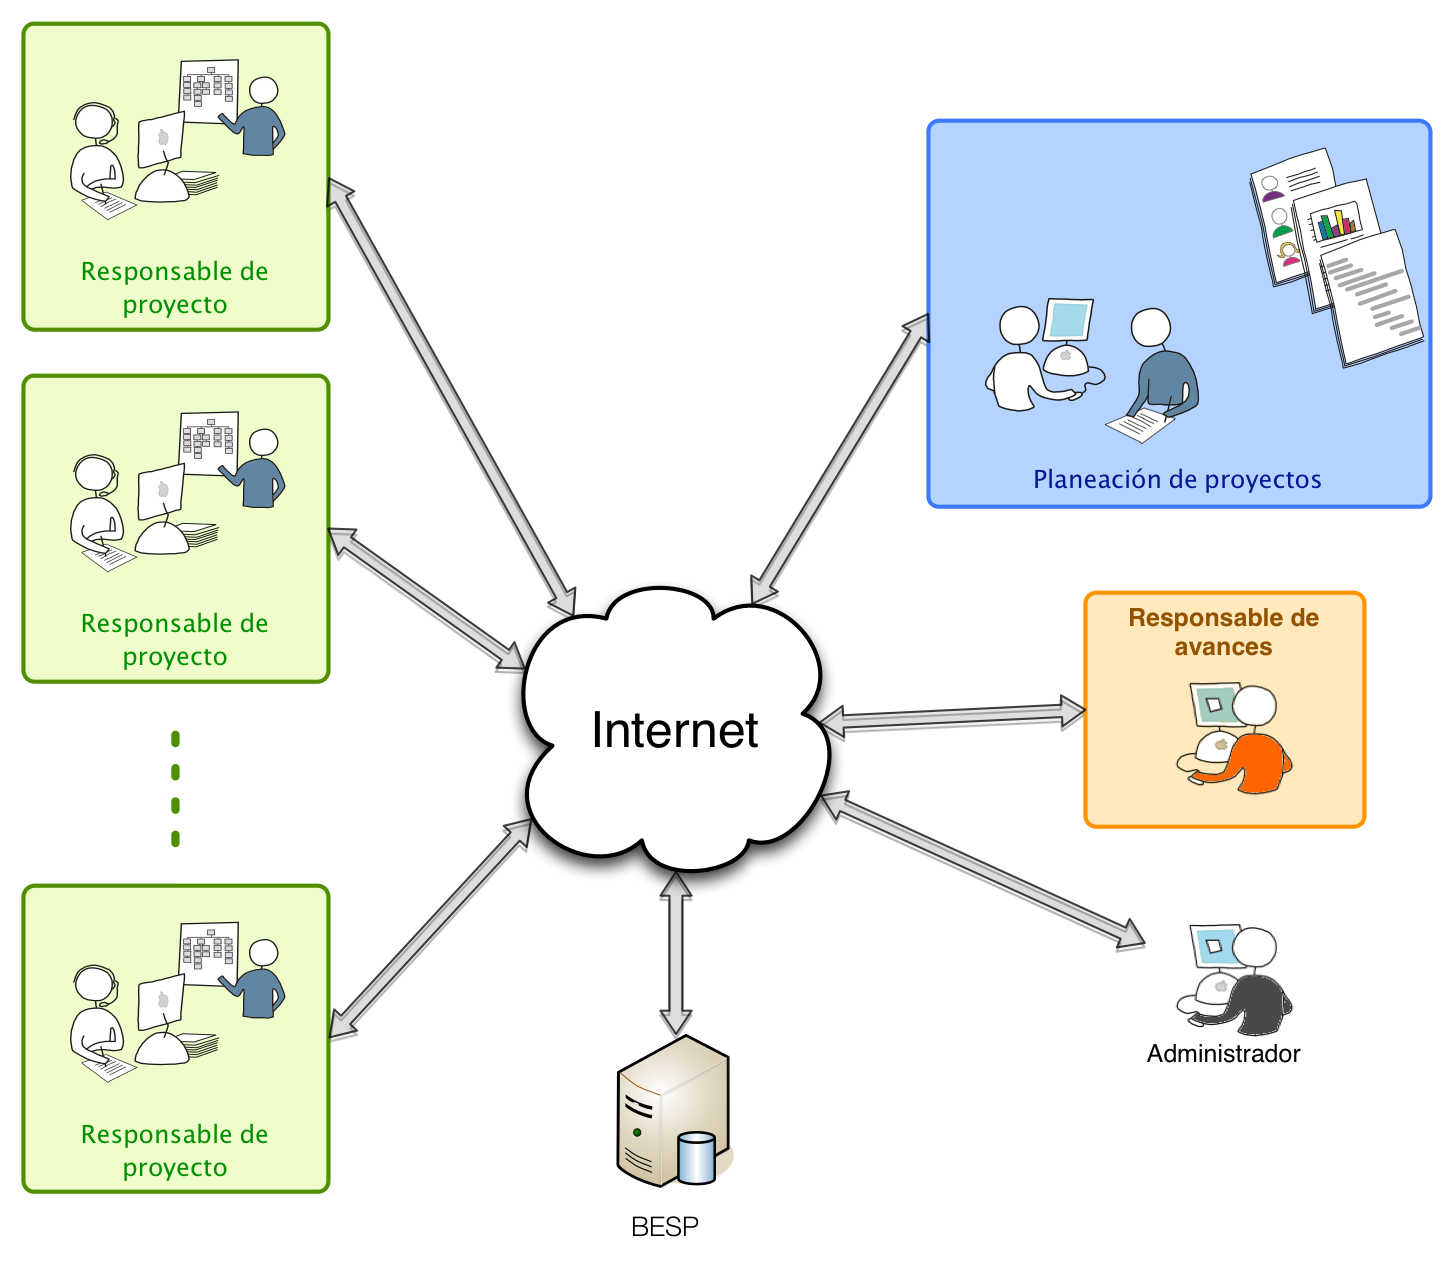
\includegraphics[width=.6\textwidth]{images/arquitectura}}
		\caption{Arquitectura del sistema.}
		\label{fig:arquitectura}
	\end{center}
\end{figure}

En la figura~\ref{fig:arquitectura} se describe la estructura del sistema, en ella se detalla ...


